\begin{frame}{Benchmark Problem}
\begin{minipage}{.4\textwidth}
% \begin{itemize}
\small{Dataset in \textit{Zhang, EDBT 2004}: no longer available,
 so we generate new benchmark problems:}
\begin{itemize}
    \onslide<2-> \item \small{All parks ($\approx 9000$) in Australia from \textit{OpenStreetMap}}
    \onslide<3-> \item \small{Use them as polygonal obstacles}
\end{itemize}
% \end{itemize}
\end{minipage}%
\begin{minipage}{.6\textwidth}
    \begin{adjustbox}{max totalsize={.9\textwidth}{.9\textheight}, right}
    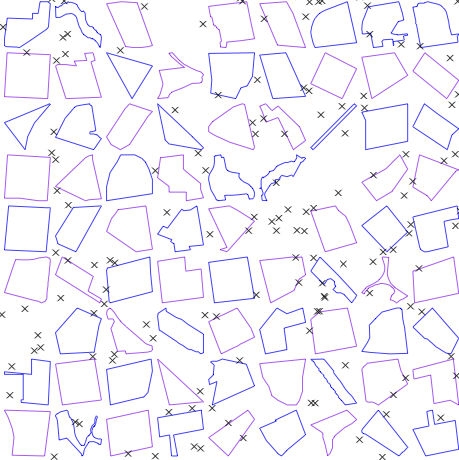
\includegraphics{pic/distribution.png}
    \end{adjustbox}
\end{minipage}
\end{frame}

\begin{frame}{Competitors}
\small{There are two types of test case:}
\begin{itemize}
    \item<1-> \small{Dense targets: $|T| \approx |O|, |O| \approx 9000$}
    \item<1-> \small{Sparse targets: $|T| <= 10, |O| \approx 9000$}
\end{itemize}
\small{In dense targets experiments, we compare between:}
\begin{itemize}
    \item<1-> \small{\textit{LVG} (from \textit{Zhang, EDBT 2004})}
    \item<1-> \small{Interval heuristic}
    \item<1-> \small{Target heuristic}
\end{itemize}
\small{In sparse targets experiments, we compare between:}
\begin{itemize}
    \item<1-> \small{burte-force Polyanya}
    \item<1-> \small{Interval heuristic}
    \item<1-> \small{Target heuristic}
\end{itemize}
\end{frame}

\begin{frame}{Dense targets}
\begin{minipage}{.5\textwidth}
    \centering
    $\scriptscriptstyle |O| \approx 9000, |T| \approx |O|, k=1$
    \begin{adjustbox}{max totalsize={.9\textwidth}{.9\textheight}, right}
    \centering
    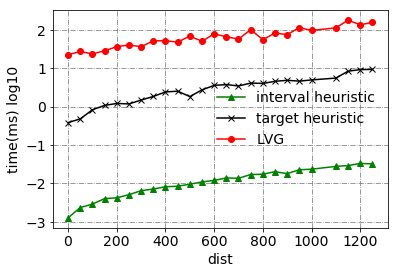
\includegraphics{pic/e1_dense_time.png}
    \end{adjustbox}
\end{minipage}%
\begin{minipage}{.5\textwidth}
    \centering
    $\scriptscriptstyle |O| \approx 9000, |T| \approx |O|, k \in [1, 10]$
    \begin{adjustbox}{max totalsize={.9\textwidth}{.9\textheight}, right}
    \centering
    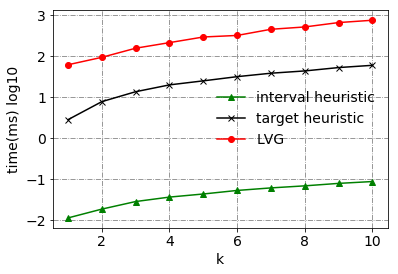
\includegraphics{pic/e2_dense_time.png}
    \end{adjustbox}
\end{minipage}
\begin{itemize}
    \item \small{\textit{Interval heuristic} is three order of magnitude faster than \textit{LVG}, in all aspects.}
\end{itemize}
\end{frame}

\begin{frame}{Sparse targets: fix $k=1$}
\centering
$\scriptscriptstyle |O| \approx 9000, |T| \in [1, 10]$
\begin{minipage}{.5\textwidth}
    \begin{adjustbox}{max totalsize={.9\textwidth}{.9\textheight}, right}
    \centering
    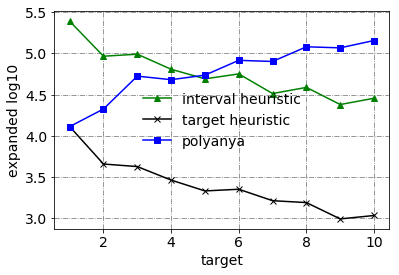
\includegraphics{pic/e3_gen.png}
    \end{adjustbox}
\end{minipage}%
\begin{minipage}{.5\textwidth}
    \begin{adjustbox}{max totalsize={.9\textwidth}{.9\textheight}, right}
    \centering
    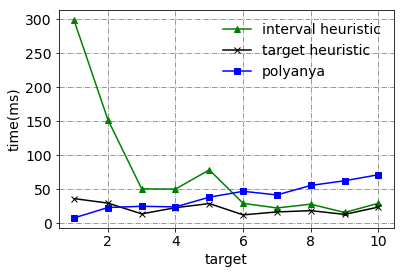
\includegraphics{pic/e3_time.png}
    \end{adjustbox}
\end{minipage}
\begin{itemize}
    \item \small{\textit{Target heuristic} always has smaller search space. (left)}
    \item \small{It gradually lose such advantage when $|T|$ increase. (right)}
    \item \small{Reason: the costly heuristic function.}
\end{itemize}
\end{frame}

\begin{frame}{Sparse targets: fix $|T|=10$}
\centering
$\scriptscriptstyle |O| \approx 9000, k \in [1, 10]$
\begin{minipage}{.5\textwidth}
    \begin{adjustbox}{max totalsize={.9\textwidth}{.9\textheight}, right}
    \centering
    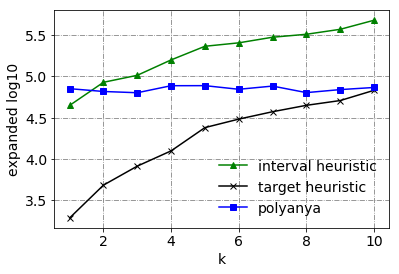
\includegraphics{pic/e2_sparse_gen.png}
    \end{adjustbox}
\end{minipage}%
\begin{minipage}{.5\textwidth}
    \begin{adjustbox}{max totalsize={.9\textwidth}{.9\textheight}, right}
    \centering
    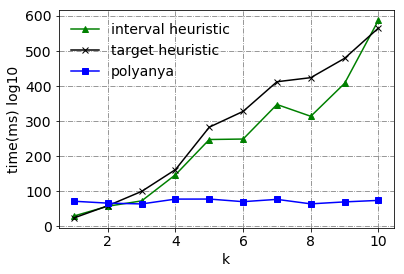
\includegraphics{pic/e2_sparse_time.png}
    \end{adjustbox}
\end{minipage}
\begin{itemize}
    \item \small{\textit{Target heuristic} always has small search space. (left)}
    \item \small{It's outperformed by \textit{brute-force Polyanya} when $k>=2$. (right)}
    \item \small{Reason: lazy reassignment becomes more frequent.}
\end{itemize}
\end{frame}
